\chapter{Application Android}\label{chap:android}

Ce chapitre décrit l’application qui embarque le modèle~: son architecture, la chaîne de traitement d’une photo, la logique de décision (seuil de confiance et conseils) et les tests effectués.

\section{Cahier des charges de l’application}

L’application doit~: (i) permettre de prendre une photo ou d’en choisir une dans la galerie~; (ii) identifier le fruit et son stade de maturité \emph{localement}, sans connexion~; (iii) afficher le résultat de façon lisible, avec le niveau de confiance et des probabilités alternatives~; (iv) éviter de présenter comme certain un résultat que le modèle ne maîtrise pas~; (v) donner un conseil pratique adapté au stade détecté.

\section{Architecture}

L’application est écrite en \textbf{Kotlin} et comporte une seule activité (\code{MainActivity}). L’interface est décrite en XML avec des composants Material 3 (cartes, boutons, indicateurs de progression linéaires). Le modèle \code{fruit\_ripeness.tflite} et le fichier \code{labels.txt} sont placés dans le dossier \code{assets}, et sont chargés au démarrage. La bibliothèque TensorFlow Lite (version 2.17.0) fournit l’interpréteur.

\begin{figure}[H]
\centering
\begin{tikzpicture}[node distance=5mm]
  \node[blkw,minimum width=28mm,minimum height=15mm] (u) {\textbf{Utilisateur}\\[-1pt]{\footnotesize photo ou galerie}};
  \node[blk,minimum width=30mm,minimum height=15mm,right=of u] (d) {\textbf{Décodage}\\[-1pt]\footnotesize ImageDecoder\\orientation EXIF};
  \node[blk,minimum width=30mm,minimum height=15mm,right=of d] (p) {\textbf{Prétraitement}\\[-1pt]\footnotesize $224{\times}224$, RGB\\float32 0--255};
  \node[blk,minimum width=30mm,minimum height=15mm,below=7mm of p,fill=navy!14] (m) {\textbf{Interpréteur TFLite}\\[-1pt]{\footnotesize image + miroir}};
  \node[blk,minimum width=30mm,minimum height=15mm,left=of m] (a) {\textbf{Moyenne (TTA)}\\[-1pt]{\footnotesize 11 probabilités}};
  \node[blkg,minimum width=28mm,minimum height=15mm,left=of a] (r) {\textbf{Affichage}\\[-1pt]\footnotesize résultat, conseil,\\top-3};
  \draw[arr] (u) -- (d); \draw[arr] (d) -- (p); \draw[arr] (p) -- (m); \draw[arr] (m) -- (a); \draw[arr] (a) -- (r);
\end{tikzpicture}
\caption{Chaîne de traitement d’une photo dans l’application.}\label{fig:android}
\end{figure}

\section{Acquisition de l’image}

\begin{itemize}
  \item \textbf{Galerie}~: le sélecteur système \code{PickVisualMedia} permet de choisir une image sans demander aucune permission de stockage.
  \item \textbf{Appareil photo}~: l’application demande à l’appareil photo du système d’écrire une photo en \emph{pleine résolution} dans un fichier privé, via un \code{FileProvider}. L’option plus simple \code{TakePicturePreview} ne renvoie qu’une miniature de faible résolution, trop pauvre pour juger la couleur et la texture d’un fruit~; nous l’avons donc écartée.
\end{itemize}

\section{Décodage et prétraitement}

L’image est décodée avec \code{ImageDecoder}, qui applique automatiquement l’orientation EXIF~: une photo prise en portrait n’est pas affichée ni analysée de travers. L’image est limitée à 1\,024 pixels sur son plus grand côté (constante \code{MAX\_DISPLAY}) pour limiter la mémoire. Elle est ensuite redimensionnée à $224\times224$ et convertie en tableau de flottants~: pour chaque pixel, les valeurs R, G, B entre 0 et 255 sont écrites dans l’ordre dans un tampon de $224\times224\times3\times4$ octets. Aucune normalisation n’est nécessaire côté Kotlin, car elle est incluse dans le modèle.

Le décodage et l’inférence s’exécutent dans un \emph{thread} séparé afin de ne pas bloquer l’interface~; le résultat est publié sur le thread principal. Un indicateur de chargement est affiché entre-temps.

\section{Test-time augmentation (TTA)}\label{sec:tta}

Pour stabiliser les prédictions, l’application classe l’image \emph{et son miroir horizontal}, puis fait la moyenne des deux vecteurs de probabilités~:
\begin{equation}
  \mathbf{p} = \tfrac{1}{2}\bigl(\mathbf{p}(\text{image}) + \mathbf{p}(\text{miroir})\bigr).
\end{equation}
Cette technique, appelée \emph{test-time augmentation}, réduit la sensibilité à l’orientation du fruit (une banane pointant à gauche ou à droite) pour un coût de calcul doublé. L’entraînement incluant déjà des retournements, le modèle y est naturellement robuste.

\section{Logique de décision}

Le modèle produit toujours une probabilité maximale, même face à un objet qui n’est pas un fruit ou une image ambiguë. Afficher telle quelle la classe prédite serait trompeur. L’application applique donc trois règles à partir des deux meilleures classes, de probabilités $p_1\ge p_2$ :

\begin{enumerate}
  \item si $p_1\ge 0{,}70$ (constante \code{CONFIDENCE\_MIN})~: le résultat est présenté comme \textbf{fiable}, avec la classe, la confiance et un conseil~;
  \item si $p_1<0{,}70$ et que les deux meilleures classes concernent le \emph{même fruit} avec $p_1+p_2\ge 0{,}85$ : le résultat est «~\textbf{entre deux stades}~» et les deux hypothèses sont affichées~; c’est le cas typique d’un fruit à cheval entre deux stades de maturité~;
  \item sinon~: le résultat est «~\textbf{Incertain}~», la meilleure hypothèse est donnée à titre indicatif, accompagnée d’une invitation à reprendre la photo (un seul fruit, bien cadré, fond uni, bonne lumière).
\end{enumerate}

La couleur de la carte de résultat suit le stade~: vert pour «~non mûr~», jaune pour «~partiellement mûr~», orange pour «~mûr~», rouge pour «~trop mûr~» ou «~pourri~», gris pour l’incertain. Les trois meilleures classes sont affichées avec des barres de progression, et le temps d’inférence est indiqué.

\begin{keybox}{Pourquoi un seuil à 70\,\% ?}
Le seuil arbitre entre deux erreurs~: afficher une réponse fausse avec assurance (grave) ou refuser de répondre à tort (agaçant). Un modèle de classification donne des probabilités qui ne sont pas parfaitement calibrées~; 70\,\% est un compromis raisonnable, fixé de façon empirique. Une évaluation systématique du seuil sur le jeu de validation (courbe exactitude/couverture) est une perspective naturelle.
\end{keybox}

\section{Conseils par stade}

À chaque classe correspond un conseil pratique affiché sous le résultat (tableau~\ref{tab:conseils}).

\begin{table}[H]
\centering
\caption{Conseils affichés par l’application selon la classe détectée.}\label{tab:conseils}
\footnotesize
\begin{tabularx}{\textwidth}{@{}p{3.2cm}X@{}}
\toprule
\textbf{Classe} & \textbf{Conseil} \\
\midrule
Banane non mûre & Laisser mûrir 3 à 5 jours à température ambiante. \\
Banane mûre & À consommer dans les 1 à 2 jours. \\
Banane trop mûre & Idéale pour un gâteau, des pancakes ou un smoothie. \\
Fraise non mûre & Une fraise ne mûrit plus après la cueillette~; attendre qu’elle rougisse sur le plant. \\
Fraise partiellement mûre & Presque prête~; plus sucrée dans 1 à 2 jours. \\
Fraise mûre & À déguster rapidement, de préférence dans les 2 jours. \\
Fraise pourrie & Abîmée ou moisie~: ne pas la manger. \\
Avocat non mûr & Encore dur~; le garder 3 à 5 jours à température ambiante. \\
Avocat partiellement mûr & Bientôt prêt~; encore 1 à 2 jours. \\
Avocat mûr & À point~; à consommer dans les 1 à 2 jours. \\
Avocat pourri & Trop mûr ou abîmé~; vérifier la chair avant de le manger. \\
\bottomrule
\end{tabularx}
\end{table}

Ces durées sont des repères généraux et non des garanties~; elles dépendent de la température et de la variété.

\section{Résultats observés}

La figure~\ref{fig:captures} montre quatre cas d’usage observés dans l’émulateur Pixel (API 37).

\begin{figure}[H]
\centering
\begin{tabular}{@{}cccc@{}}
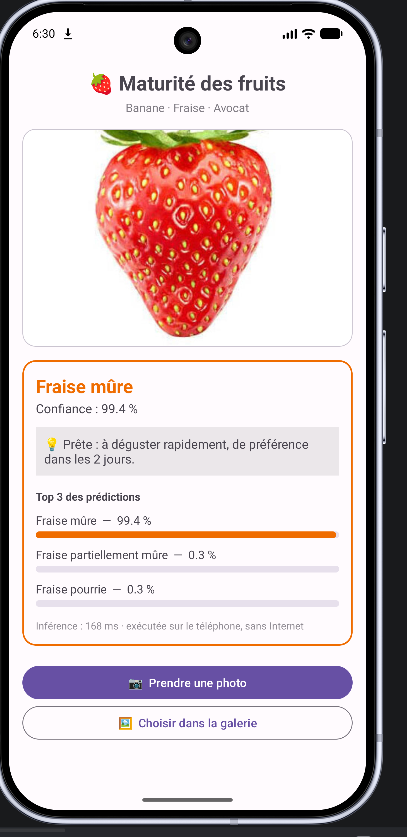
\includegraphics[height=7.0cm]{figures/app_fraise.png} &
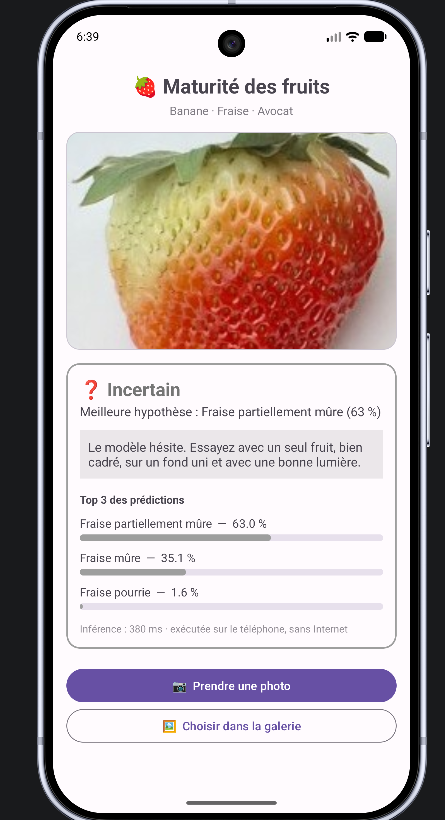
\includegraphics[height=7.0cm]{figures/app_fraise_incertain.png} &
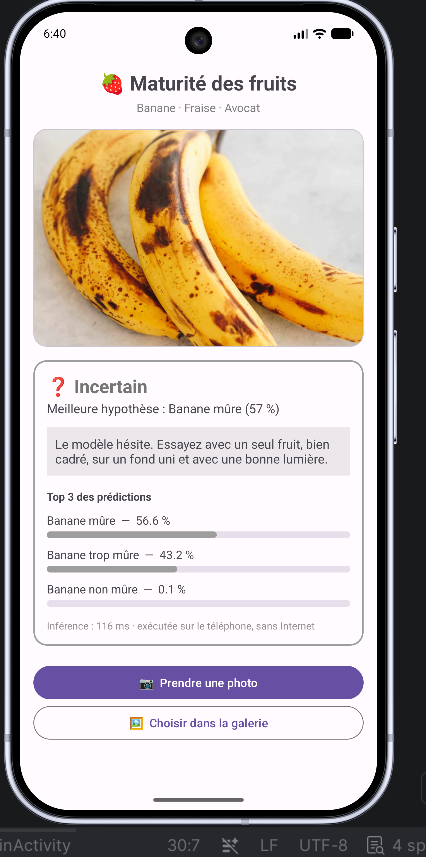
\includegraphics[height=7.0cm]{figures/app_bananes_incertain.png} &
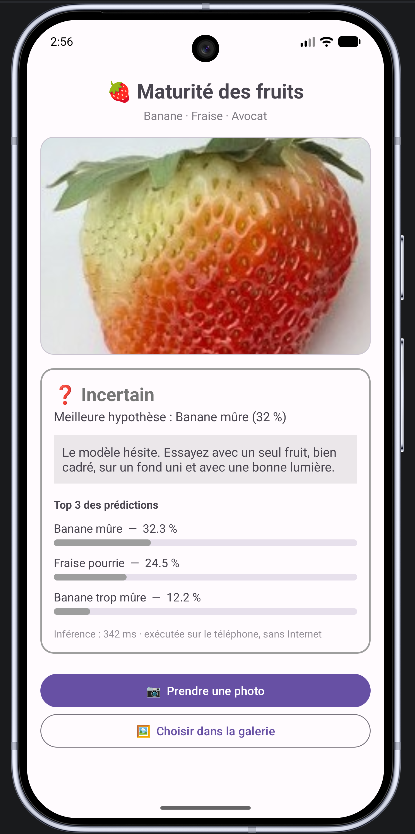
\includegraphics[height=7.0cm]{figures/app_cas.png} \\
{\scriptsize (a)} & {\scriptsize (b)} & {\scriptsize (c)} & {\scriptsize (d)}
\end{tabular}
\caption{Captures de l’application~: (a) fraise mûre reconnue avec 99,4\,\% de confiance ; (b) fraise à 63\,\%, marquée « Incertain » ; (c) bananes à 57\,\%, « Incertain » ; (d) fraise partiellement mûre d’une photo web : le meilleur score (32\,\%) va à « Banane mûre » et l’application déclare l’image incertaine.}\label{fig:captures}
\end{figure}

\begin{itemize}
  \item Dans le cas (a), un fruit isolé, bien éclairé, est reconnu à 99,4\,\% en 168\,ms.
  \item Dans les cas (b) et (c), le fruit est reconnu mais avec une confiance sous le seuil~: l’application évite d’affirmer et suggère de reprendre la photo.
  \item Le cas (d) est le plus instructif~: une fraise partiellement mûre photographiée dans un contexte très différent des données d’entraînement met le modèle en difficulté (un mauvais fruit en tête, avec 32\,\% seulement). Sans le seuil de confiance, l’application aurait annoncé « Banane mûre » ; c’est précisément le rôle de la classe « Incertain ».
\end{itemize}

\section{Points d’attention techniques}

\begin{itemize}
  \item \textbf{Orientation des photos}~: sans prise en compte de l’orientation EXIF, une photo prise en portrait serait analysée couchée. \code{ImageDecoder} règle ce point.
  \item \textbf{Qualité de la photo}~: la capture en pleine résolution passe par un \code{FileProvider}, qui donne à l’appareil photo du système le droit d’écrire dans un fichier privé de l’application.
  \item \textbf{Mémoire}~: les photos modernes (12 millions de pixels et plus) saturent la mémoire si on les décode entièrement~; d’où la limite à 1\,024 pixels.
  \item \textbf{Cohérence modèle/application}~: l’ordre des étiquettes et l’échelle des pixels (0--255) doivent correspondre exactement à ceux de l’entraînement.
  \item \textbf{Hors distribution}~: un objet qui n’est pas un fruit est tout de même classé. Le seuil limite le problème sans le supprimer (voir chapitre~\ref{chap:discussion}).
\end{itemize}

\section{Limites de l’application}

L’application suppose \textbf{un seul fruit par image}, car le modèle est un classifieur et non un détecteur. Elle ne gère que trois fruits et onze stades. Les tests ont été faits sur émulateur et sur quelques photos~; une campagne de tests sur plusieurs téléphones physiques n’a pas été réalisée.
